\subsection{Dimensiones}

\begin{figure}[h] \centering
	\centering
	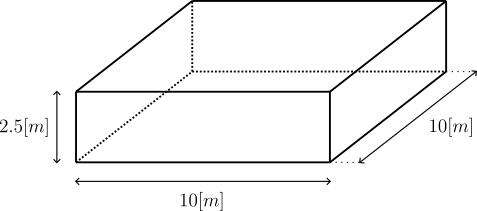
\includegraphics[width=1\textwidth]{./capitulos/resultados_discusion/images/modelo_vivienda.png}
	\caption{Vivienda modelo.}
	\label{fig:modelo_vivienda}
\end{figure}

Consideramos un modelo de vivienda simple con una única habitación de planta
cuadrada con $100[m^2]$ de área. Techo plano.

Las paredes son de $2.5[m]$ de alto, por lo tanto con una extesión total de
$100[m^2]$. De los cuales 25 son ventanas y los otros 75 son pared.

El volumen es de $100[m^2] \cdot 2.5[m] = 250[m^3]$, con
tan solo aire en su interior, que tiene una densidad de
$1.1614[kg \cdot m^{-3}]$, y pesará:

\begin{equation}
	m_{aire} = 1.1614 \cdot 250 = 290.35[kg]
\end{equation}



\subsection{Transmitancias térmicas de la vivienda}

La transmitancia térmica de las ventanas se extrae de la ficha técnica para un
modelo
\footnote{\url{https://www.veka.es/wp-content/uploads/2020/03/softline-70-doble-junta-linea-recta-por-paginas.pdf}},
que muestra (figura \ref{fig:window_tranmittance}) sus medidas de transmitancia
para el marco (frame), vidrio (glass) y global (window). Escogiendo el vidrio
de baja emisividad (BE) y relleno de argón, tenemos un valor de
$1.4\left[\frac{W}{m^2 \cdot K}\right]$, que asumimos engloba las perdidas por
conducción, convección y radiación.

\begin{figure}[h] \centering
	\centering
	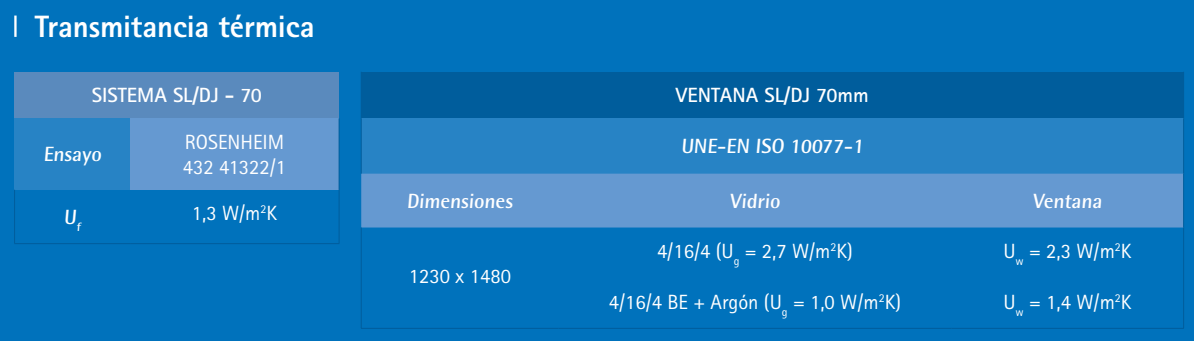
\includegraphics[width=1\textwidth]{./capitulos/resultados_discusion/images/window_transmittance.png}
	\caption{Transmitancias térmicas para ventana Veka softline 70.}
	\label{fig:window_tranmittance}
\end{figure}


Tanto paredes como techo tienen un aislamiento de $20[cm]$ de espesor de lana
de roca. Y con el dato de la conductividad térmica de este material obtenida de
la tabla de propiedades físicas en Incropera et al.
\cite{incropera1996fundamentals}, se calcula la transmitancia térmica por
conducción de un metro cuadrado de este aislamiento como


\begin{equation}
	U_{lana-roca} = \frac{k}{l} = \frac{0.049\left[\frac{W}{m \cdot K}\right]}{0.2[m]} = 0.245 \left[\frac{W}{m^2 \cdot K}\right]
\end{equation}

Pero además de pérdidas por conducción, consideramos la transferencia por
convección y radiación, tomando los datos para una superficie no reflejante
(con emisividad de 0.9) de la tabla \ref{tab:building_surface_transmittances}
obtenida de ASHRAE \cite{refrigerating2009ashrae}.

\begin{table}[ht]
	\centering
	\caption{Resistencia y conductancia para aire y superficies de edificios con $\epsilon = 0.9$}
	\label{tab:building_surface_transmittances}
	\begin{tabular}{llcc}
		\toprule
		\textbf{Position of Surface}       & \textbf{Direction of Heat Flow} & $h_i$ & $R$   \\
		\midrule
		\textbf{Still Air}                 &                                 &       &       \\
		Horizontal                         & Upward                          & 9.26  & 0.11  \\
		Sloping at 45°                     & Upward                          & 9.09  & 0.11  \\
		Vertical                           & Horizontal                      & 8.29  & 0.12  \\
		Sloping at 45°                     & Downward                        & 7.50  & 0.13  \\
		Horizontal                         & Downward                        & 6.13  & 0.16  \\
		\midrule
		\textbf{Moving Air (any position)} &                                 &       &       \\
		Wind (for winter) at 6.7 m/s       & Any                             & 34.0  & 0.030 \\
		Wind (for summer) at 3.4 m/s       & Any                             & 22.7  & 0.044 \\
		\bottomrule
	\end{tabular}
\end{table}


Con estos datos calculamos las transmitancias de paredes y techo como:

\begin{equation}
	\frac{1}{U} = \frac{1}{h_{pared-interior}} + \frac{1}{U_{lana-roca}} + \frac{1}{h_{pared-exterior}}
\end{equation}

tomando como $h_{pared-exterior}$ la media entre los dos datos dados, de verano
e invierno:

\begin{equation}
	\frac{1}{U_{paredes}} = \frac{1}{8.29} + \frac{1}{0.245} + \frac{1}{28.35} \rightarrow U_{paredes} = 0.2359 \left[\frac{W}{m^2 \cdot K}\right]
\end{equation}

\begin{equation}
	\frac{1}{U_{techo}} = \frac{1}{9.26} + \frac{1}{0.245} + \frac{1}{28.35} \rightarrow U_{techo} = 0.2366 \left[\frac{W}{m^2 \cdot K}\right]
\end{equation}


\subsection{Suelo radiante}

Por simplicidad, consideramos un único circuito con tubo de polietileno reticulado (PEX) de 1
pulgada que lleva unas dimensiones asociadas mostradas en la figura
\ref{fig:1_inch_pex}.
Aunque en la práctica es más común la instalación de varios circuitos (e.g.
uno para cada habitación), cada uno con diámetros de tubo menores.

\begin{figure}[h] \centering
	\centering
	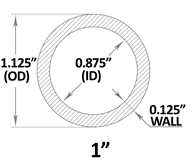
\includegraphics[width=0.3\textwidth]{./capitulos/resultados_discusion/images/1_inch_pex.png}
	\caption{Dimensiones de un tubo PEX de una pulgada. Fuente: \url{https://www.pexuniverse.com/pex-tubing-technical-specs}.}
	\label{fig:1_inch_pex}
\end{figure}


Para el espaciado entre pasos de tubo, se adopta una convención establecida
\footnote{\url{https://www.blueridgecompany.com/articles/PEX_tube_sizing_spacing}},
seleccionando una distancia de 18" (redondeando a $50[cm]$) entre pasos. La
configuración en zig-zag permite determinar la longitud total del tubo (figura
\ref{fig:esquema_tubos_suelo}). Que puede observarse es de $H = 21 \cdot 10 + 10 =
220[m]$.

Y el área de los tubos viene dada por la longitud total de estos $H$, y el
perímetro exterior del tubo.

\begin{equation}
	A_{tubos} = 2 \pi R_{ext} H = 2 \pi \cdot 0.0142875 \cdot 220 = 19.7[m^2]
\end{equation}


\begin{figure}[h] \centering
	\centering
	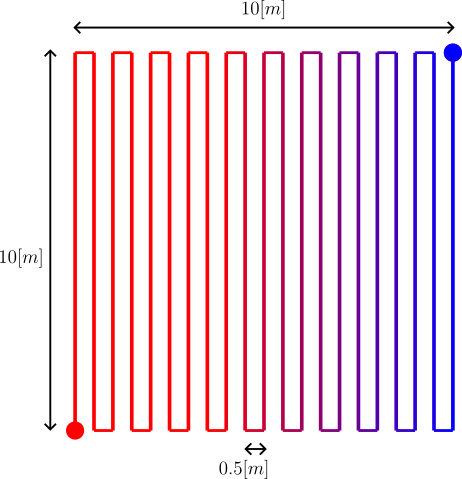
\includegraphics[width=0.6\textwidth]{./capitulos/resultados_discusion/images/esquema_tubos_suelo.png}
	\caption{Suelo radiante, configuración zig-zag. 220 metros de longitud.}
	\label{fig:esquema_tubos_suelo}
\end{figure}

De nuevo hemos optado por un arreglo simple para facilitar los cálculos,
pero también es común el patrón de espiral, mostrado en la figura \ref{fig:spiral_pattern_floor},
que distribuye el calor de forma más uniforme por el suelo, aunque con una buena
conductividad del material de la losa que integra los tubos (hormigón), las diferencias de
temperaturas en distintas partes de la habitación deberían de ser poco perceptibles.

\begin{figure}[h] \centering
	\centering
	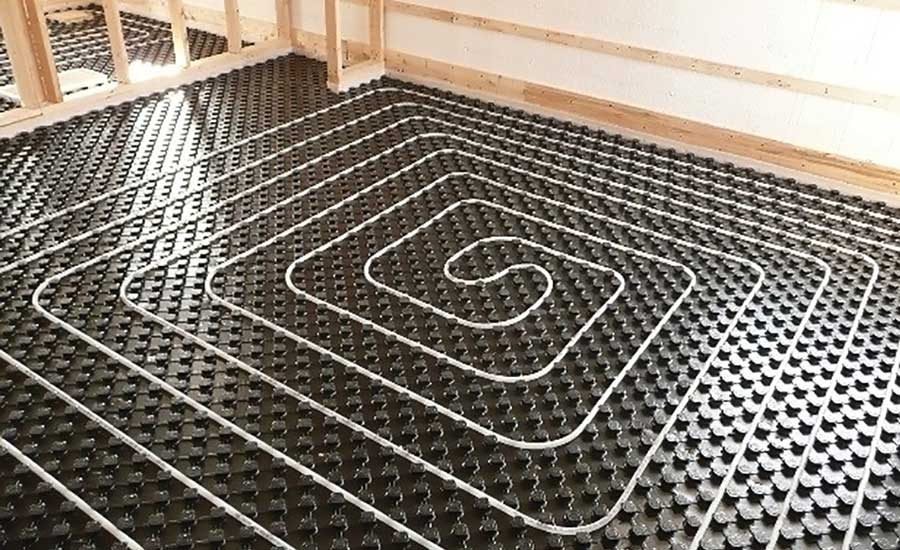
\includegraphics[width=1\textwidth]{./capitulos/resultados_discusion/images/spiral_pattern_floor.jpg}
	\caption{Tubos para suelo radiante en configuración espiral. Fuente: \url{https://www.achrnews.com/articles/141245-hydronics-offer-unique-options-for-residential-heating}.}
	\label{fig:spiral_pattern_floor}
\end{figure}

La losa de hormigón que da una inercia térmica considerable al suelo, se ha
tomado de 5cm. Y tampoco hemos considerado que se haya recubierto la losa de
hormigón con ningún azulejo, porcelánico o madera.

Con una densidad del hormigón de $2300[kg\cdot m^{-3}]$, la masa de esta losa es:

\begin{equation}
	m_{suelo} = 100[m^2] \cdot 0.05[m] \cdot 2300[kg\cdot m^{-3}] = 11500[kg]
\end{equation}


\subsection{Paneles solares}

Ya que disponemos de un techo de $100[m^2]$, y cada kW de paneles solares
requiere de un área de aproximadamente $5[m^2]$, como se muestra en el SAM
(figura \ref{fig:solar_panel_area}), como mucho podremos instalar $20[kW]$ de
potencia solar.

\begin{figure}[h] \centering
	\centering
	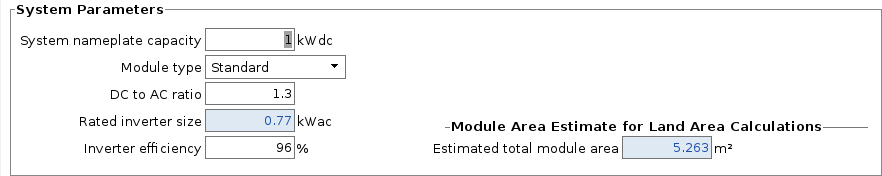
\includegraphics[width=1\textwidth]{./capitulos/resultados_discusion/images/solar_panel_area.png}
	\caption{Área de $5.263[m^2]$ para $1[kW]$ de panales solares instalados. Datos obtenidos de SAM (System Advisor Model).}
	\label{fig:solar_panel_area}
\end{figure}
